\documentclass[compress,red]{beamer}
%\mode<presentation>
\usetheme{CambridgeUS}

\usepackage{epsfig}

%frame formula:
%% \frame{\frametitle{TITLE MISSING}
%% \begin{enumerate}
%% \item
%% \end{enumerate}
%% }


\title{MEng thesis status}
\author{Oscar Moll}
\date{\today}
\institute{?}

\newcommand{\code}{\ttfamily}
\useoutertheme[subsection=false]{smoothbars}

\begin{document}
\frame{
	\titlepage
}

\section[Outline]{}
\frame{\tableofcontents}

\section{System description}

\frame{\frametitle{Service interface}
  \begin{enumerate}
  \item update: {\code putEdge(vertexV, vertexW, metadata)}
  \item queries: 
  \item edge query: {\code metadata = getEdge(vertexV, vertexW)}
  \item fanout query: {\code list<Vertex>, newcursor = getFanout(vertex, inward/outward, maxResults, cursor)}
  \item intersection: {\code list<Vertex>, newcursor = getIntersection(vertexV, inwardV/outwardV, vertexW, inwardW/outwardW, maxResults, cursor)}
  \item Also: counts, set difference, union. etc.
  \end{enumerate}
}

\frame{\frametitle{Other service info}
\begin{itemize}
\item  Focus on live updates and simple queries compared to graph data systems
used for more offline write/graph traversal queries.

\item  Data distributed across several 10's of nodes to be able to satisify throughput requirements, as well as space.

\item Data store o keeps vertex relations and edge data only, not node data nor
message tables. Hence using the graph to keep neighbors together is not a big gain.
\end{itemize}
}

%of many connectons being symmetric  (can consolidate?)
%effect of tentatively placing adjacent nodes together: can consolidate 4 edge strcutrues in the best case.
%indexing?
%my implementation

\section{Motivation for approaches}

\subsection{Solution background}

\frame{\frametitle{main partitioning options}
\begin{enumerate}
\item Range partitioning: good for scans, suffers when vertex very large. Involves remembering limits.
\item Hash Partitioning: on vertex, good for scans, still suffers from vertex very large. Easy to remember.
\item Hash Partitioning on edge endpoints: good for writes, rest become all-shards queries.
\item Hash Partitioning (hybrid):  the more it ameliorates worst cases the less optimal for users with few followers.
\item Fine Grained, lookup table options: need to solve problem of storing routing information.
\item Arbitrary partitining plus one hop replication. space overhead explodes thanks to graph properties. (sketchy reasoning here)
\end{enumerate}
}

\subsection{Related work I am using}
\frame{\frametitle{related problems}
\begin{enumerate}
\item Many systems dealing with graphs simply hash by vertex (eg. Giraph), current Twitter graph store. 
\item Graphs of this kind often exhibit high skew degree distributions.
\item Skew issue signifficant enough also addressed in other graph processing systems, eg. GraphLab talk on Monday.
\end{enumerate}
}

\frame{\frametitle{some techniques}
\begin{enumerate}
\item Schism paper proposes technique for partitioning to minimize distributed transactions
\item In my case, no transactions, but still relevant to minimize related communication overhead, esp when nodes 
can have large degrees.
\item Fine grained partitioning paper can be done on at least some `heavy' subset of the graph. Or even more, if we are willing
to take one round of communication (eg DHT index?)
\item Collocation (with replication) of edges of adjacent nodes. excessive replication? (and also charges more on writes). May address
intersection queries if there is correlation  between actual graph and intersection graph
\item The problem of optimal partitioning of data based on size vs. communication tradeoff also touched in DeWitt `Hybrid-range partitioning' paper. 
\end{enumerate}
}

\frame{\frametitle{more surveying}
\begin{enumerate}
\item Heuristics of cheap, online graph repositioning also present in literature. 
\item Many focus on keeping the graph {\em itself} clustered, which is helful for Tweet delivery when receiver tweet table is
in the same location as senders, but not necessarily for intersection
\item Some mention `partition by country' or other simple techniques, but this information not available in this case.
\item Some papers related in the sense of using case by case reasoning on members of graph to successfully optimize overall system. Eg. Feeding frenzy.
\end{enumerate}
}


\section{Main proposal}

\subsection{Approach}

\frame{\frametitle{Approach}
\begin{enumerate}
\item Focus on each individual operation by itself (though some approaches help several)
\item Focus on latency of operations, though throughput itself should not be penalized.
\item Focus on using knowledge about specific workload and data to improve performance for that specific case.

\item Not considering replication based techniques (testing them requires also considering the consequences for update operations)
\end{enumerate}
}

\subsection{Fanouts}
\frame{\frametitle{Fanout queries}
Large variation in degree size means queries to some vertices
entail much more work than queries to others.

Latency is affected by two effects: one related to communication one to amount of work.

\[L = max_{i=1}^n(L_i) + qd/n \]

$L$ is latency, $L_i$ is latency for an individual server to return, $d$ is degree, $q$ is some system dependent constant, $n$ is the number of servers distributing the work.

If $d$ is small, $L$ is mostly from communication $max_{i=1}^n(L_i)$. If $d$ is large the cost comes mostly from the actual work $qd/n$. In $max_{i=1}^n(L_i)$ grows with $n$, whereas $qd/n$ decreases with it.
}

\frame{\frametitle{Two tiers}

Hence the optimal choice depends on the degree. Can choose to optimize for the distribution (DeWitt)

Or, get the best of both worlds and treat nodes of large degree differently than nodes of small degree.

More complicated now, because need to remember how to treat each id. Data has power law distribution:

The memory cost of remembering is $O(\mbox{\# high degree vertices})$ the benefits are $O(\mbox{\# of {\em edges} in high degree vertices})$. 

So it is possible to remember only a few vertices. This is the two-tier strategy.

Exactly where to draw the cutoff and how to partition needs tuning. 
}


\frame{\frametitle{Best possible world savings}

\begin{figure}
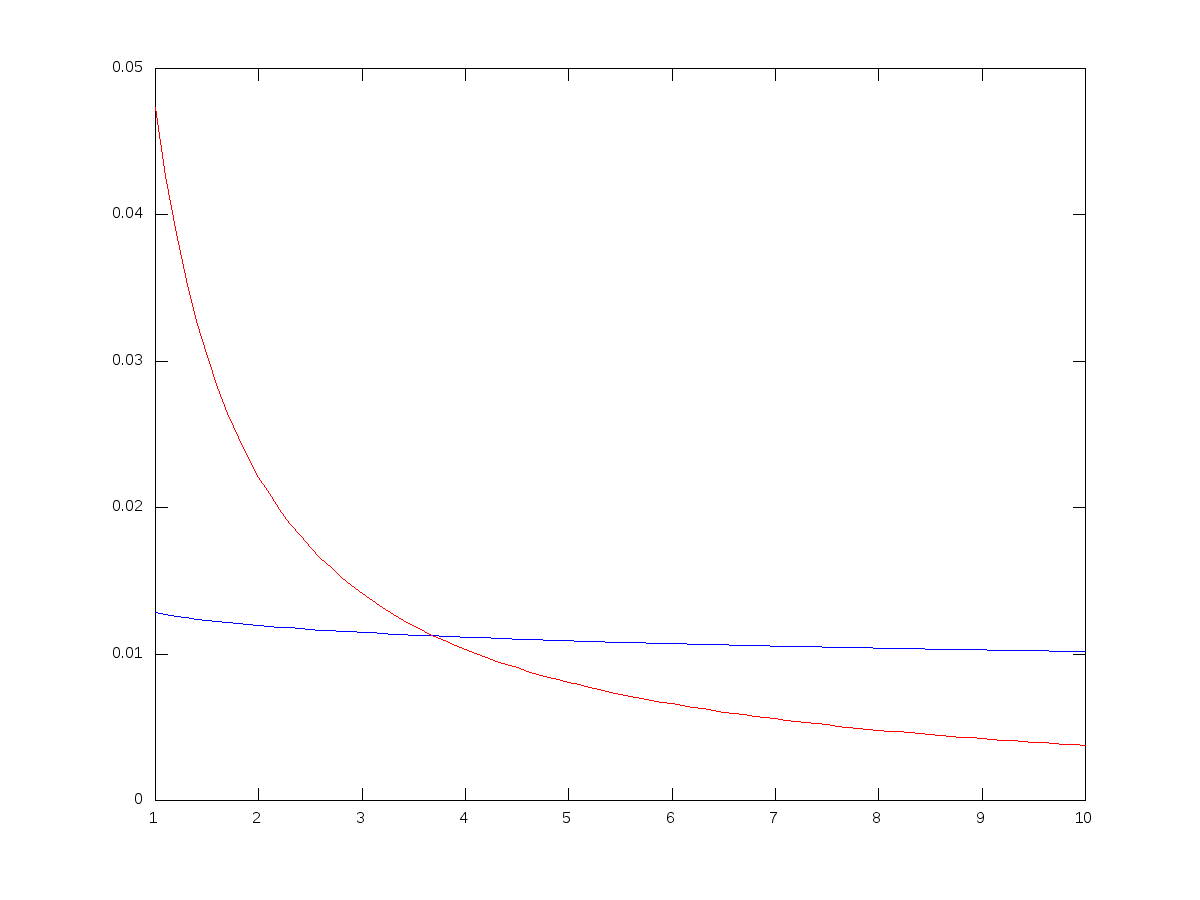
\includegraphics[width=4in]{vertexVsDegree2.png}
\end{figure}

} 

\frame{\frametitle{Savings with actual graph parameters}

\begin{figure}
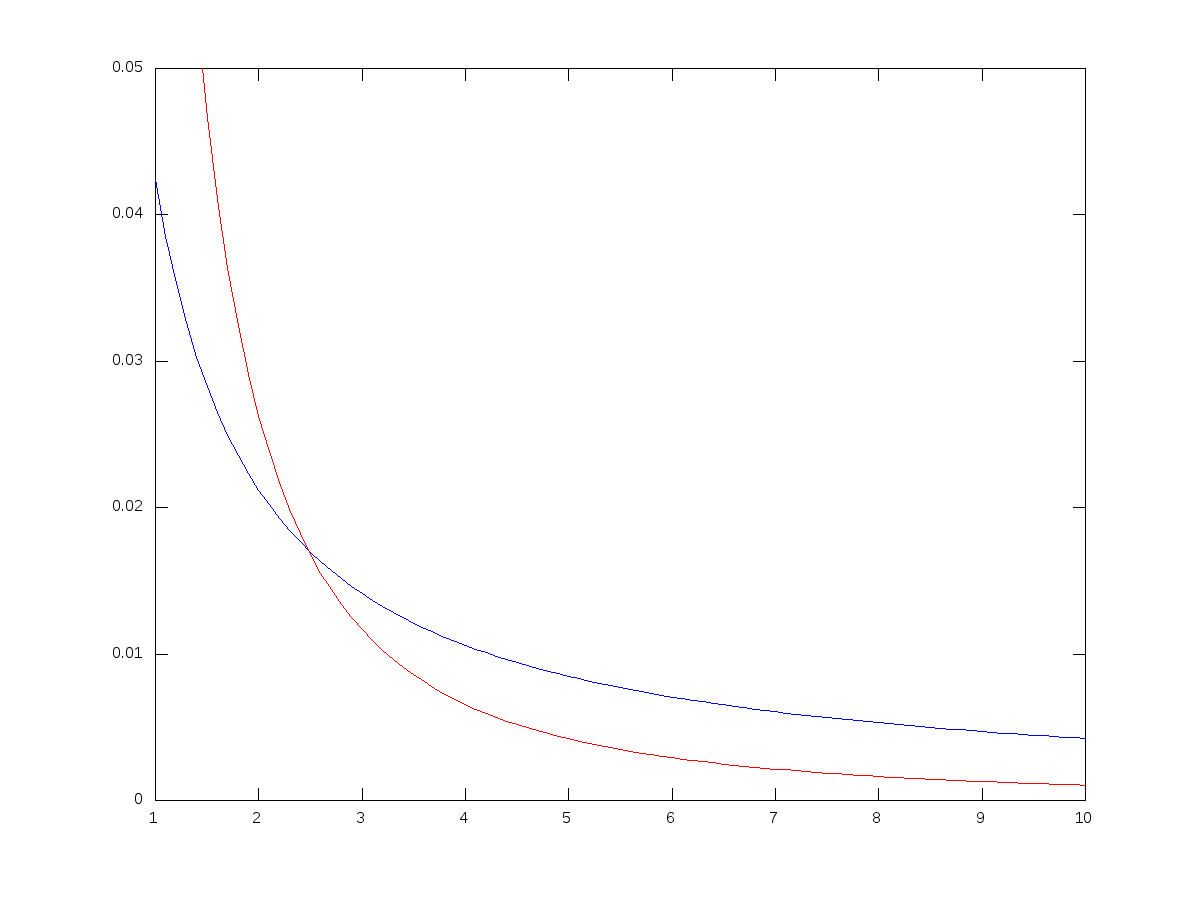
\includegraphics[width=4in]{vertexVsDegree.png}
\end{figure}

}


\subsection{Intersection}

\frame{\frametitle{Intersection queries}
For intersections, variation in degree still an issue for latency variability, 
but there are oportunities for optimization. Since intersection has a filtering effect, it is best to give as high priority as possible to it.

\begin{enumerate}
\item An intersection cannot be larger than the smaller set, so if a set is small, it is worth pushing the operation to the node with the larger set rather than moving the large set at all.

\item Another strategy is collocating data from two sets we know are intersected often. (based on the Schism paper)

\item  Independent of the other optimizations, splitting large fanout vertices into several machines could enable parallelism in intersection.

\end{enumerate}

Of those optimizations, I attempted to apply the ideas from the Schism paper on this context. 

Applying parallelism gets complicated by the {\code maxResults} and {\code offset} arguments to the operation, as well as order constraints on the interface.

}

\section{Experiments and results}

\subsection{real data (goal of being at Twitter)}
\frame{\frametitle{Graph}

{\em (See graph)}

\begin{enumerate}
\item Twitter data = graph snapshot + actual query logs 
\item Graph \~ 100 million users, 5 billion directed edges. (snapshot from some time ago).
\item Degree distribution: both indegree and outdegree have power law shaped dist 
with coeff about 1.8, 2.1 respectively. Larger coeff means less extreme degrees.
\item Max indegree in snapshot was ~ 1 million, avg ~ 40, min ~ 1.
\end{enumerate}
}
%lots of repeated edges. 8 billion after removing duplicates from 10 billion.
%plots, indeg vs. outdeg.

\frame{\frametitle{Logs}
\begin{enumerate}
\item fanout(vertex, inward/outward, small, -1)  70\%. (ie, asking for the first follower). Did not log inward/outward.
\item fanout(vertex, inward/outward, between 1000 and 5000, -1) 10\%
\item intersection: 1.5\%
\item edges: 0.5\%
\item not included in log: counts, writes.
\end{enumerate}
}
%more info at flockdb github
%how do these graph's evolve, what problems will become more striking.
%workload and graph
\subsection{results with real data}

\frame{\frametitle{Results on Twitter Data}
\vspace{0.25cm}

{\em (See graph)}

\begin{enumerate}

\item three main methods for fanout queries: all shards (in this case only 5 though), two-tier ( ie above 20k deg all shards, below, one shard), vertex hash (control)
\item and three for intersection: workload driven (graph partitioning based on historic log), all-shards, vertex.
\item short story: methods visibly improve latency and show expected effects, 
\item caveat: tuning error means I did not use two-tier optimally. 
\item caveat: intersections training set and testing set were the same. (needed to sanity check it worked in that case)
\end{enumerate}

}

%now plots.

\subsection{Synthetic data}
\frame { \frametitle{Synthetic benchmark description}
\begin{enumerate}
\item generate graphs and workload
\item use power law number generator to make more realistic
\item for graph, power law degree distribution.
\item for workload, power law in frequence of queries to different nodes (access skew)
\item important: can experiement with different skew parameters, unlike with real data.
\item other parameters: number of queries, ratio of max to min degree, avg degree, number of vertices.
\item single threaded, only useful for measuring pure operation and communication latency..
\end {enumerate}
}

\subsection{Results with synthetic data}

\frame { \frametitle{Results}
\begin{enumerate}
\item The ones shown in December meeting (via skype)
  \begin{enumerate}
  \item Curve of latency vs. num shards for split  is u-shaped.
  \item optimal number of shards depends on \# followers, 
  \end{enumerate}
\item used to tune two tier for the real workload.
\item In the past, pointed out I should develop model. Also, pointed out suspicions on small
 speedup.
\item found a possible reason for that, but late. 
\item can run again without need for data. (need to regenerate those particular plots anyway)
\end {enumerate}
}

\section{Work done}

\subsection{last 5 months}
\frame { \frametitle{system}
\begin{enumerate}
\item Constructed basic model of system in Java (interfaces, parallel requests etc)
\item Set up RMI for client to server comm (data nodes)
\item Loading (for real data, logs)
\item Benchmark and graph generation (synthetic)
\item Data formating and analysis in Pig (real data)
\item Data display in Octave.
\item Configuration system (for easier benchmarking)
\item Optimization to fit real data (more efficient data structures, load process, serialization)
\item 4k lines of java, 2k lines of java tests, 0.5k of pig.
\item Some building work came to nothing, some was reinventing the wheel.
\item Getting METIS working, reformating data when it didn't
\item Debugging plots that made no sense
\end {enumerate}
}

\subsection{issues}
\frame{ \frametitle{issues}
\begin{enumerate}
\item Only got to do limited experiements with real data.
\item Not evaluating writes: No concurrency overhead in measurements.
\item Not evaluating other strategies (like replication based ones, because they involve large modifications to system)
\item perhaps should have used larger query graph (over longer time), so that larger fraction represented.
\item Need to replay synthetic benchmark. (need machines?)
\item moving nodes is static.
\end{enumerate}

}

\subsection{pending}
\frame{\frametitle{ideas for further work}

Higher priority:
\begin{enumerate}

\item work on the cost model approach to tuning two-tier
\item with that, repeat synthetic data experiments, need to figure out where.
\item writing first draft, getting feedback, getting aproval. dates?

\end{enumerate}

Low priority:
\begin{enumerate}
\item other operations? eg more general set operations.
\item to explore other ideas partitioning, using synthetic benchmarks.
\item cacheing as an approach to exploiting statistical regularity?
\item think of metis algorithm, maybe it could be made into online algorithm.
\end{enumerate}
}

\end{document}
